In this section, we examine the effective frequency response induced by translation via each method as a function of source azimuth.
As described in \secref{sec:06_Simulation_Framework:Azimuth_Dependence}, for these simulations, we let $L_\text{in} = 4$, pick $u = 0.25$~m and $s_0 = 2.5$~m (so $\gamma = 10$), and translate to $\vec{r}_0 = (0, 0, 0)$.
Based on the findings discussed above, here we use beamforming with $Q = N_\text{in} = 25$ for the plane-wave translation method.

The induced frequency responses are plotted in \figref{fig:07_Characterization_Extrapolation:Azimuth_Dependence}.
From \figref{fig:07_Characterization_Extrapolation:Azimuth_Dependence:PWT}, we see that the plane-wave translation method introduces sporadic notches in the frequency response of the signal, which do not appear to follow any obvious pattern.
Otherwise, however, the frequency responses are largely flat for all source azimuths.
This is in agreement with the finding of \citet[cf.~Figs.~7c and 7f]{HahnSpors2015b}: that the induced frequency responses are largely flat under critically-sampled conditions, i.e., when the number of plane-wave terms matches the number of ambisonics signals.

\begin{figure*}[t]
    	\centering
    	\begin{subfigure}[b]{0.49\textwidth}
        		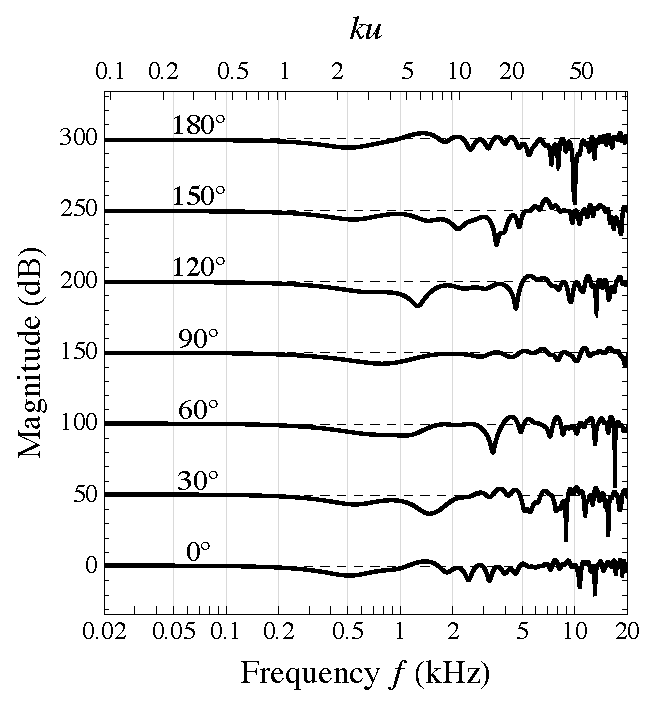
\includegraphics[width=\textwidth]{07_characterization_extrapolation/figures/sourceAz_freqResp_pwt.eps}
        		\caption{Plane-wave translation}
        		\label{fig:07_Characterization_Extrapolation:Azimuth_Dependence:PWT}
    	\end{subfigure}
	\hfill
    	\begin{subfigure}[b]{0.49\textwidth}
        		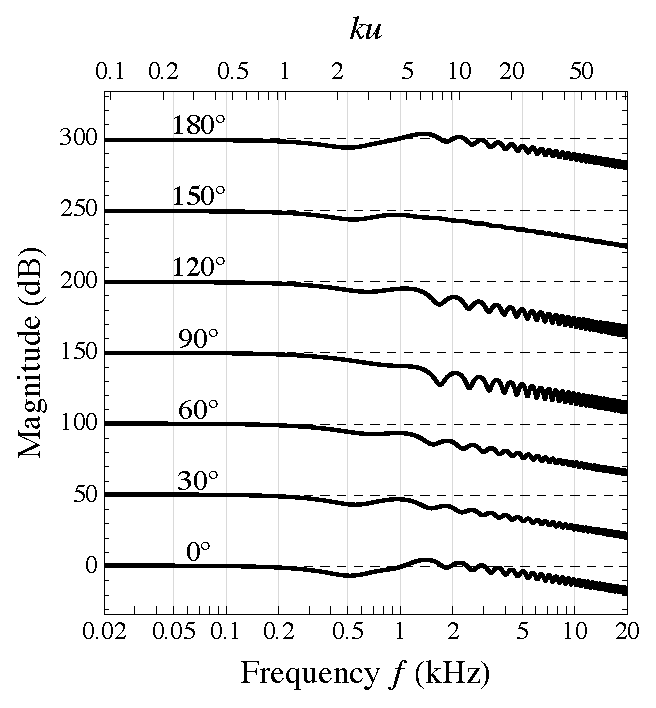
\includegraphics[width=\textwidth]{07_characterization_extrapolation/figures/sourceAz_freqResp_sre.eps}
        		\caption{Ambisonics translation}
        		\label{fig:07_Characterization_Extrapolation:Azimuth_Dependence:SRE}
    	\end{subfigure}
	
	\caption[Magnitude responses across azimuths for each extrapolation method.]{
	Magnitude responses caused by the plane-wave and ambisonics translation methods for various source azimuths.
  The bottom axes show frequency in kHz while the top axes show the nondimensional frequency $ku$ for a microphone distance of $u = 0.25$~m.
  For legibility, each frequency response is offset by $50$~dB and the responses have been artificially truncated (where needed) to not exceed $-45$~dB.}
	\label{fig:07_Characterization_Extrapolation:Azimuth_Dependence}
\end{figure*} %%NOTE%% vertical axis label is too complicated: |A0 / B0ref| or something

We also note from \figref{fig:07_Characterization_Extrapolation:Azimuth_Dependence:PWT} that the frequency response for a source azimuth of $90^\circ$ is particularly flat, which suggests that translation perpendicular to the direction of the source introduces very little spectral coloration.
This appears to contradict another finding of \citet{HahnSpors2015b}: that translation parallel to the source direction introduces less coloration than translation perpendicularly.
However, their finding was only shown for oversampled conditions, where $Q > N_\text{in}$ \citep[cf.~Fig.~7]{HahnSpors2015b}; for critically-sampled conditions (where $Q = N_\text{in}$), as considered here, the induced coloration is apparently smaller (albeit not nearly as significantly so) for perpendicular translations.

As shown in \figref{fig:07_Characterization_Extrapolation:Azimuth_Dependence:SRE}, the ambisonics translation method introduces a high-frequency roll-off, which does not depend on source azimuth.
Recall from \secref{sec:03_Navigation_Techniques:SR_Technique}, however, that the corner frequency of this roll-off does vary proportionally to $L_\text{in} / \| \vec{r}_0 - \vec{u} \|$.
Consequently, we expect the spectral coloration induced by this method to increase steadily with increasing translation distance, while the overall level will steadily decrease.